\documentclass{article}
\usepackage[utf8]{inputenc}
\usepackage{graphicx}
\usepackage{grffile}
\usepackage{amsmath}
\usepackage{amssymb}
\usepackage{bm}

\title{Bent Marshak Waves - Hurricane \& Hammer}
\author{Yuval Kochavi}
\date{January 2025}

\begin{document}

\maketitle

\section{Introduction}
\begin{itemize}
    \item Radiation-driven heat waves (Marshak waves) appear in HEDP, ICF, and astrophysical systems.
    \item Classical Marshak theory describes 1D planar diffusion with $\sqrt{t}$ scaling.
    \item Experiments show curved radiation fronts in foam targets.
    \item Curvature is caused primarily by energy loss into surrounding walls.
    \item \textbf{Goal: derive an analytic 2D model for bent Marshak waves with lossy boundaries.}
\end{itemize}

\section{Boundaries Problem}

\subsection*{Physical setup}
\begin{itemize}
    \item 2D planar slab geometry - working in Cartesian coordinates $(x,y)$.
    \item Constant temperature source $T_s$ at $x=0$.
    \item Radiation front at $x = x_F(y,t)$.
    \item Lossy walls at $y=\pm L$ with albedo $a$ - constant over time in the article.
    \item The article derive the model assuming LTE, meaning $T_{rad} = T_{mat} = T$ (black).
    \item Another stong assumption is that the energy ($e$) and opacity ($\kappa$) are constant in $T$.
    \item The fundumental equation is:
    \begin{equation}
        \rho\frac{\partial e}{\partial t} = \frac{4}{3}\boldsymbol{\nabla} \cdot \left(\frac{1}{\kappa\rho}\boldsymbol{\nabla} (\sigma_{SB}T^4)\right)
    \end{equation}
    \begin{figure}[h!]
    \centering
    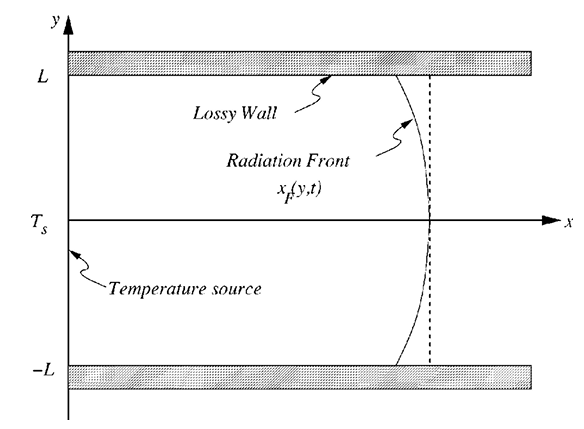
\includegraphics[width=0.5\textwidth]{figures_for_summeries/hurricane.png}
    \caption{The physical setup of a bent Marshak wave propagating in a 2D slab with lossy walls - Cartesian coordinates $(x,y)$.}
    \label{fig:physical_setup}
    \end{figure}
\end{itemize}

\subsection*{Governing equation}
\begin{itemize}
    \item Supersonic assumption: material motion negligible, meaning the material stays in place over times scales of interest, so $\rho$ is constant in time and space.
    \item Quasi-steady assumption: time derivative small compared to spatial diffusion, so $\partial_t e$ negligible.
    \item Radiation diffusion equation reduces to:
    \[
    \nabla^2 T^4 = 0
    \]
    \item Temperature field expanded in eigenmodes - Laplace equation in Cartesian coordinates.
    \item General solution:
    define $u = T^4$ then we get $\nabla^2 u = u_{xx}+u_{yy}=0$. Using separation of variables $u(x,y) = X(x)Y(y)$ we get:
    \[\frac{X''(x)}{X(x)} = -\frac{Y''(y)}{Y(y)} = k^2\]
    So we get:
    \[X(x) = A e^{kx} + B e^{-kx}\]
    \[Y(y) = C \cos(ky) + D \sin(ky)\]
    Therefore the general solution is (knowing the problem symmetry around $y=0$):
    \begin{equation}
    T^4(x,y) = \sum_{n=0}^\infty \left[A_n e^{k_n x} + B_n e^{-k_n x}\right] \cos(k_n y)
    \end{equation}
    Notice that the heat-wave front depends only on $y$ and $t$, and knowing the y-symmetry we can write it as:
    \begin{equation}
    x_F(y,t) = \sum_{n=0}^\infty c_n(t) \cos(k_n y)
    \end{equation}
    where $x_F$ defined by the place where $T(x_F,y,t) = 0$, and so he shares the same eigenvalues $k_n$ as the temperature field.
\end{itemize}

\subsection*{Wall boundary condition}
\begin{itemize}
    \item Nonideal wall introduces energy loss. Radiation flux $F_{in}$ arrives, but only a fraction $a$ is reflected back as $F_{out} = a F_{in}$. Therefore the flux at the wall is:
    \begin{equation*}
    F_{wall} = F_{in} - F_{out} = (1-a) F_{in}
    \end{equation*}
    Now, knowing that $F_{in} = \sigma_{SB} T^4$, we get:
    \begin{equation*}
    F_{wall} = (1-a) \sigma_{SB} T^4
    \end{equation*}
    But also, from fick's law we know that:
    \begin{equation*}
    F_{wall} = \boldsymbol{F} \cdot \hat{y} = -\frac{4}{3\kappa\rho} \frac{\partial (\sigma_{SB} T^4)}{\partial y}
    \end{equation*}
    Equating the two expressions for $F_{wall}$ we get the boundary condition at $y=\pm L$:
    \begin{equation}
    \frac{\partial T^4}{\partial y}|_{y=\pm L} = \frac{3}{4} \kappa \rho (a-1) T^4|_{y=\pm L}
    \end{equation}
    Notice that since $a<1$ we have $(a-1)<0$ meaning that the derivative is negative, so the temperature decreases towards the wall, as expected.
\end{itemize}

\subsection*{Eigenmode expansion}
\begin{itemize}
    \item Radiation temperature expanded as:
    \[
    T^4(x,y) = \sum_n \cos(k_n y)\left[A_n(t)e^{k_n x} + B_n(t)e^{-k_n x}\right]
    \]
    Spatial derivative:
    \[
    \frac{\partial T^4}{\partial y} 
    = - \sum_n k_n \sin(k_n y)\left[A_n e^{k_n x} + B_n e^{-k_n x}\right]
    \]
    Substitution of mode expansion gives:
    \[
    - k_n \sin(k_n L) = \frac{3}{4}\rho\kappa (a-1)\cos(k_n L)
    \]
    Rearranged to:
    \begin{equation}
    \tan(k_n L) = \frac{\varepsilon}{k_n L}
    \end{equation}
    Definition of small parameter:
    \[
    \varepsilon = \frac{3}{4}(1-a)\tau
    \]
    where $\tau = \rho\kappa L$ is the optical depth.

    \item Solutions are intersections of: $y = \tan(k_n L)$ and $y = \dfrac{\varepsilon}{k_n L}$. For small $\varepsilon$:
    \[
    k_n L \approx n\pi
    \]
    with small corrections.
    \end{itemize}

    \subsubsection*{Physical meaning of $\varepsilon$}
    \begin{itemize}
    \item Interpretation:
    \[
    \varepsilon \sim 
    \frac{\text{energy lost sideways per diffusion step}}
    {\text{energy transported forward}}
    \]
    \item Regimes:
    \begin{itemize}
        \item $\varepsilon \ll 1$ : weak wall losses $\Rightarrow$ nearly 1D Marshak wave
        \item $\varepsilon \sim 1$ : strong lateral losses $\Rightarrow$ strong bending
    \end{itemize}
    \end{itemize}

    \subsubsection*{Constraint on albedo}
    \begin{itemize}
    \item Small-parameter condition:
    \[
    \varepsilon < 1 \;\;\Rightarrow\;\; a > 1 - \frac{4}{3\tau}
    \]
    \item For typical $\tau \sim 3$:
    \[
    a > 1 - \frac{4}{9} \approx 0.56
    \;\;\Rightarrow\;\;
    \frac{2}{3} \lesssim a < 1
    \]
    \item Meaning: theory valid only for \textbf{high-albedo walls}.
    \end{itemize}

\subsection*{Eigenvalue expansion}

From the wall boundary condition (Eq. 5), we write the eigenvalues as perturbations around the ideal values:
\begin{equation}
\tan(k_n L) = \frac{\varepsilon}{k_n L},
\end{equation}
with small correction $\phi_n \ll 1$.

Using the Taylor expansion,
\begin{equation}
\tan(n\pi + \phi_n) \simeq \phi_n + \frac{1}{3}\phi_n^3 + \mathcal{O}(\phi_n^5),
\end{equation}
the eigenvalue equation becomes
\[
\phi_n + \frac{1}{3}\phi_n^3 \simeq \frac{\varepsilon}{n\pi + \phi_n}.
\]

To leading order, this gives the quadratic approximation
\[
\phi_n^2 + n\pi \phi_n - \varepsilon \simeq 0,
\]
with solution
\begin{equation}
\phi_n \simeq \frac{-n\pi + \sqrt{n^2\pi^2 + 4\varepsilon}}{2}.
\end{equation}

Expanding the square root,
\[
\sqrt{n^2\pi^2 + 4\varepsilon}
\simeq n\pi\left(1 + \frac{2\varepsilon}{n^2\pi^2} - \frac{2\varepsilon^2}{n^4\pi^4} + \cdots \right),
\]
we obtain
\begin{equation}
\phi_n \simeq \frac{\varepsilon}{n\pi} - \frac{\varepsilon^2}{n^3\pi^3} + \mathcal{O}(\varepsilon^3),
\end{equation}
and for the lowest mode:
\begin{equation}
\phi_0 = \sqrt{\varepsilon}.
\end{equation}

The mode amplitudes are expanded in powers of $\varepsilon$:
\begin{equation}
A_n = A_n^{(0)} + \sqrt{\varepsilon}\,A_n^{(1/2)} + \varepsilon A_n^{(1)} + \cdots,
\end{equation}
\begin{equation}
B_n = B_n^{(0)} + \sqrt{\varepsilon}\,B_n^{(1/2)} + \varepsilon B_n^{(1)} + \cdots.
\end{equation}
The goal is to solve for the coefficients $A_n^{(i)}$, $B_n^{(i)}$ order-by-order, using the boundary conditions at the source and front.

\subsection*{Source boundary condition ($x=0$, $T=T_s$)}
Let's assume \textbf{constant source temperature $T_s$} at $x=0$:
\[
T_s^4 = T^4(0,y) = \sum_n \left[A_n + B_n\right] \cos(k_n y).
\]
Using
\[
\cos(k_n y) = \cos\!\left(\frac{n\pi y}{L} + \frac{\phi_n y}{L}\right),
\]
and expanding:
\[
\cos(\alpha+\beta)=\cos\alpha\cos\beta-\sin\alpha\sin\beta,
\]
we get:
\[\cos(k_n y) =
\cos\!\left(\frac{n\pi y}{L}\right)
\cos\!\left(\frac{\phi_n y}{L}\right)
-
\sin\!\left(\frac{n\pi y}{L}\right)
\sin\!\left(\frac{\phi_n y}{L}\right).
\]
with small-angle expansions for $\phi_n$, we can use tylor expansions:
\[
\cos\!\left(\frac{\phi_n y}{L}\right) \approx 1 - \frac{(\phi_n y)^2}{2L^2} + \frac{(\phi_n y)^4}{24L^4} + \mathcal{O}(\phi_n^6)
\]
\[
\sin\!\left(\frac{\phi_n y}{L}\right) \approx \frac{\phi_n y}{L} - \frac{(\phi_n y)^3}{6L^3} + \mathcal{O}(\phi_n^5)
\]

Substituting back, we get:
\[
\cos(k_n y) \approx
\cos\!\left(\frac{n\pi y}{L}\right)
\left[1 - \frac{(\phi_n y)^2}{2L^2} + \frac{(\phi_n y)^4}{24L^4}\right]
- \sin\!\left(\frac{n\pi y}{L}\right)
\left[\frac{\phi_n y}{L} - \frac{(\phi_n y)^3}{6L^3}\right].
\]
Substituting the expansions for $A_n$, $B_n$, and $\cos(k_n y)$ into the source boundary condition, we collect terms order-by-order in $\varepsilon$.
At zeroth order:
\[
\sum_n \left[A_n^{(0)} + B_n^{(0)}\right] \cos\!\left(\frac{n\pi y}{L}\right) = T_s^4.
\]
Using orthogonality of cosine functions, we find:
\begin{equation}
A_n^{(0)} + B_n^{(0)} =
\begin{cases}
T_s^4, & n=0,\\
0, & n>0,
\end{cases}
\end{equation}
At order $\sqrt{\varepsilon}$, we have (since $\phi_0 \sim \sqrt{\varepsilon}$ and $\phi_{n>0} \sim \varepsilon$):
\[
\sum_n \left[A_n^{(1/2)} + B_n^{(1/2)}\right] \cos\!\left(\frac{n\pi y}{L}\right) = 0,
\]
leading to:
\begin{equation}
A_n^{(1/2)} + B_n^{(1/2)} = 0.
\end{equation}
At order $\varepsilon$:
\begin{equation}
    %split in the middle for better readability
    \begin{split}
        0 = \sum_n \left(\varepsilon\left[A_n^{(1)} + B_n^{(1)}\right] \cos\!\left(\frac{n\pi y}{L}\right)
        - \left[A_n^{(0)} + B_n^{(0)}\right]\frac{(\phi_n y)}{L}\sin\!\left(\frac{n\pi y}{L}\right)\right) \\
        - \varepsilon\frac{y^2}{2L^2}\left[A_0^{(0)} + B_0^{(0)}\right].
    \end{split}
\end{equation}
But since $sin(0)=0$ and $A_{n>0}^{(0)} + B_{n>0}^{(0)}=0$, the second term vanishes, leaving:
\[
\sum_n \left[A_n^{(1)} + B_n^{(1)}\right] \cos\!\left(\frac{n\pi y}{L}\right)
= \frac{y^2}{2L^2} T_s^4.
\]
Now using orthogonality again, we find:
\begin{equation}
A_n^{(1)} + B_n^{(1)} =
\begin{cases}
\displaystyle \frac{T_s^4}{3}, & n=0,\\[6pt]
\displaystyle \frac{2(-1)^n T_s^4}{n^2\pi^2}, & n>0.
\end{cases}
\end{equation}
Notice that, 
\[
\int_{-L}^{L} y^2 \cos\!\left(\frac{n\pi y}{L}\right) dy =
\begin{cases}
\displaystyle \frac{2L^3}{3}, & n=0,\\[6pt]
\displaystyle \frac{4(-1)^n L^3}{n^2\pi^2}, & n>0.
\end{cases}
\]

Thus,
\[
A_n + B_n =
\begin{cases}
T_s^4\!\left(1+\frac{\varepsilon}{3}\right) + \mathcal{O}(\varepsilon^{3/2}), & n=0,\\[6pt]
\displaystyle \frac{4(-1)^n \varepsilon T_s^4}{n^2\pi^2} + \mathcal{O}(\varepsilon^{3/2}), & n>0.
\end{cases}
\]

\subsection*{Front boundary condition ($T(x_F,y)\approx 0$)}
\textbf{The problem:} the front position $x_F(y,t)$ is unknown a priori, and the temperature must vanish there:
\[
T^4(x_F,y) = 0.
\]
We use a \textbf{weak-curvature approximation}, assuming the front is nearly planar with small transverse perturbations:
\[
\delta x(y,t) \sim \mathcal{O}(\varepsilon).
\] 
Using Eq. 3, we write:
\begin{equation}
x_F(y,t) = c_0(t) + \delta x(y,t),
\end{equation}
with
\begin{equation}
\delta x(y,t) = \sum_{n\ge1} c_n(t)\cos(k_n y).
\end{equation}

Taylor expanding the temperature around $x=c_0(t)$:
\begin{equation}
T^4(x_F,y) \approx T^4(c_0,y) + (x_F-c_0)\,\partial_x T^4|_{c_0}.
\end{equation}
But, the LHS must vanish for all $y$, so to leading order we impose:
\[
T^4(c_0,y) \approx [c_0 - \sum_{n=0}^\infty c_n \cos(k_n y)]\,\partial_x T^4|_{c_0} = 0.
\]
Or equivalently,
\[
T^4(c_0,y) = -\sum_{n=1}^\infty c_n \cos(k_n y)\,\partial_x T^4|_{c_0}.
\]

Using the mode expansion
\[
T^4(x,y) = \sum_n \cos(k_n y)\left(A_n e^{k_n x} + B_n e^{-k_n x}\right),
\]
we define
\[
D_n(x) \equiv A_n e^{k_n x} + B_n e^{-k_n x}.
\]

Thus,
\[
T^4(c_0,y) = \sum_n D_n(c_0)\cos(k_n y),
\]
\[
\partial_x T^4(c_0,y) = \sum_n k_n\cos(k_n y)
\left(A_n e^{k_n c_0} - B_n e^{-k_n c_0}\right).
\]

\subsubsection*{order by order front condition}

The physical front condition is
\[
T(x_F,y) \approx 0,
\]
which implies, at leading order,
\[
T^4(c_0,y) = \mathcal{O}(\varepsilon).
\]

Therefore,
\begin{equation}
D_n^{(0)}(c_0) = A_n^{(0)}e^{k_n c_0} + B_n^{(0)}e^{-k_n c_0} = 0.
\end{equation}
And similarly for $\mathcal{O}(\sqrt{\varepsilon})$:
\begin{equation}
D_n^{(1/2)}(c_0) = A_n^{(1/2)}e^{k_n c_0} + B_n^{(1/2)}e^{-k_n c_0} = 0.
\end{equation}

This gives the fundamental relation:
\[
A_n^{(0)} = - B_n^{(0)} e^{-2k_n c_0}.
\]
And similarly for $\mathcal{O}(\sqrt{\varepsilon})$:
\[
A_n^{(1/2)} = - B_n^{(1/2)} e^{-2k_n c_0}.
\]

At the next order, $\mathcal{O}(\varepsilon)$, we have (same derivation as we did for the source BC with the orders):
\begin{equation}
    %split in the middle for better readability
    \begin{split}
        \varepsilon \sum_{n=0}^\infty \Bigl(
        \varepsilon\left[A_n^{(1)}e^{k_n c_0} + B_n^{(1)}e^{-k_n c_0}\right] \cos\!\left(\frac{n\pi y}{L}\right)
        \\ - \left[A_n^{(0)} e^{k_n c_0} + B_n^{(0)}e^{-k_n c_0}\right]\frac{(\varepsilon y^2)}{2L^2}
        \Bigr) \\
        = - c_1 \cos\!\left(\frac{\pi y}{L}\right) \frac{\sqrt{\varepsilon}}{L} \left[A_0^{(0)} e^{k_0 c_0} + B_0^{(0)}e^{-k_0 c_0}\right] \cos\left(\frac{\sqrt{\varepsilon}}{L} y\right).
    \end{split}
\end{equation}
The second term vanishes due to the leading-order front condition, using orthogonality we get:
\begin{equation}
    A_m^{(1)} e^{k_m c_0} + B_m^{(1)} e^{-k_m c_0} =
    \begin{cases}
        -c_1 \frac{\sqrt{\varepsilon}}{L\pi^2}\left(A_0^{(0)} e^{k_0 c_0} - B_0^{(0)}e^{-k_0 c_0}\right), & n=0,\\[6pt]
        -c_1 \frac{(-1)^m \sqrt{\varepsilon} \pi (1+m^2)}{L(m-1)^2(m+1)^2}\left(A_0^{(0)} e^{k_0 c_0} - B_0^{(0)}e^{-k_0 c_0}\right), & n>0.
    \end{cases}
\end{equation}
And this is right to order $\mathcal{O}(\varepsilon)$. Since the RHS is $\mathcal{O}(\sqrt{\varepsilon})$, we can use the leading-order front condition to write:

\begin{equation}
A_n e^{k_n c_0} + B_n e^{-k_n c_0} = 0 + \mathcal{O}((\varepsilon)^{3/2}),
\end{equation}
which implies that the curvature corrections enter only at order $\mathcal{O}((\varepsilon)^{3/2})$. Furthermore, this yields the fundamental relation:
\[ 
A_n = - B_n e^{-2k_n c_0} + \mathcal{O}((\varepsilon)^{3/2}).
\]

Define
\[
S_n \equiv A_n + B_n.
\]

One can then solve for $A_n$, $B_n$:
\[
B_n = \frac{S_n e^{k_n c_0}}{2\sinh(k_n c_0)}, 
\qquad
A_n = -\frac{S_n e^{-k_n c_0}}{2\sinh(k_n c_0)}.
\]

Hence,
\[
A_n e^{k_n x} + B_n e^{-k_n x}
= - S_n \frac{\sinh[k_n(x-c_0)]}{\sinh(k_n c_0)}.
\]

Substituting the previously derived coefficients:

\[
S_n =
\begin{cases}
T_s^4\!\left(1+\dfrac{\varepsilon}{3}\right) + \mathcal{O}(\varepsilon^{3/2}), & n=0,\\[8pt]
\dfrac{4(-1)^n \varepsilon T_s^4}{n^2\pi^2} + \mathcal{O}(\varepsilon^{3/2}), & n>0,
\end{cases}
\]

gives:
\begin{equation}
    A_n e^{k_n x} + B_n e^{-k_n x} =
    \begin{cases}
        - T_s^4 (1+\frac{\varepsilon}{3}) \frac{\sinh(k_0(x-c_0))}{\sinh(k_0 c_0)}, & n=0,\\[6pt]
        -c_1 \frac{4(-1)^n \varepsilon T_s^4}{n^2\pi^2}\frac{\sinh(k_0(x-c_0))}{\sinh(k_0 c_0)}, & n>0.
    \end{cases}
\end{equation}
 
And finally, the reconstructed temperature field is
\begin{equation}
\begin{split}
\frac{T^4(x,y)}{T_s^4}
&=
-\left(1+\frac{\varepsilon}{3}\right) \cos\!\left(\frac{\sqrt{\varepsilon}}{L}y\right) \frac{\sinh[k_0(x-c_0)]}{\sinh(k_0 c_0)} \\
&\quad+ \frac{4\varepsilon}{\pi^2} \sum_{n=1}^{\infty} \frac{(-1)^{n+1}}{n^2} \cos(k_n y)\, \frac{\sinh[k_n(x-c_0)]}{\sinh(k_n c_0)} + \mathcal{O}(\varepsilon^{3/2}).
\end{split}
\end{equation}

At first glance, it may seem atrange to see $varepsilon$ both in the eigenvalues $k_n$ and as a prefactor in the expansion. However, this gives the write boundary condition at the source:
\[
\frac{T}{T_s}^4 \bigg|_{y=0} = 1+ \frac{\varepsilon}{3} + \frac{4\varepsilon}{\pi^2}\sum_{n=1}^\infty \frac{(-1)^{n+1}}{n^2} = 1,
\]
where we used the fact that $\sum_{n=1}^\infty \frac{(-1)^{n+1}}{n^2} = -\frac{\zeta(2)}{2} = -\frac{\pi^2}{12}$.


\section{Front Equation of Motion}

The dynamics of the radiation front are obtained from local energy balance at the front.  
The physical statement is:

\begin{quote}
\emph{Energy density $\times$ front velocity = radiative energy flux into the front.}
\end{quote}

Mathematically,
\begin{equation}
\rho e \, \dot{x}_F(y,t) \;=\; F_{\text{rad}}(x_F),
\end{equation}
where $\rho e$ is the volumetric internal energy of the cold material, and the radiative flux is given by diffusion theory:
\begin{equation}
F_{\text{rad}} \;=\; -\frac{4\sigma}{3\kappa\rho}\,\nabla T^4.
\end{equation}

Evaluated at the front, this gives
\begin{equation}
\rho e\, \dot{x}_F(y,t)
\;=\;
-\frac{4\sigma}{3\kappa\rho}\,
\partial_x T^4\big|_{x=x_F}.
\label{eq:front_balance}
\end{equation}

This equation is the fundamental evolution law for the radiation front.

\subsection{Mode expansion of the front}

We expand the front position in transverse eigenmodes:
\begin{equation}
x_F(y,t) = \sum_{n=0}^{\infty} c_n(t)\cos(k_n y),
\end{equation}

The time derivative is therefore
\begin{equation}
\dot{x}_F(y,t) = \sum_{n=0}^{\infty} \dot{c}_n(t)\cos(k_n y).
\end{equation}

\subsection{Evaluation of the radiative flux}

From the reconstructed temperature field,
\[
T^4(x,y) = \sum_n \cos(k_n y)\left(A_n e^{k_n x} + B_n e^{-k_n x}\right),
\]
the longitudinal gradient is
\begin{equation}
\partial_x T^4
=
\sum_n k_n \cos(k_n y)\left(A_n e^{k_n x} - B_n e^{-k_n x}\right).
\end{equation}

Evaluating at $x=x_F$ and using the weak-curvature approximation
\[
x_F(y,t) \approx c_0(t) + \mathcal{O}(\varepsilon),
\]
we obtain to leading order
\begin{equation}
\partial_x T^4\big|_{x_F}
\;\approx\;
\sum_n k_n \cos(k_n y)\,
\left(A_n e^{k_n c_0} - B_n e^{-k_n c_0}\right).
\end{equation}

\subsection{Evolution equations for the front modes}

Substituting into the front balance equation \eqref{eq:front_balance} and projecting onto each transverse mode using orthogonality, we obtain a system of evolution equations:

\paragraph{Zeroth mode ($n=0$):}
\begin{equation}
\dot{c}_0(t)
=
\frac{D_M}{2}\left(1+\frac{\varepsilon}{3}\right)
\frac{\sqrt{\varepsilon}}{L\sinh\!\left(\frac{\sqrt{\varepsilon}}{L}c_0\right)}\,
+ \mathcal{O}(\varepsilon^2).
\label{eq:c0_evol}
\end{equation}

\paragraph{Higher modes ($n\ge1$):}
\begin{equation}
\dot{c}_n(t)
=
\frac{D_M}{2}\,
\frac{4\varepsilon}{\pi^2}
\frac{(-1)^{n}}{n^2}
\frac{k_n}{\sinh(k_n c_0)}
+ \mathcal{O}(\varepsilon^2).
\label{eq:cn_evol}
\end{equation}

Defining the classical Marshak diffusion constant
\begin{equation}
D_M \;\equiv\; \frac{8\sigma T_s^4}{3\kappa\rho^2 e},
\end{equation}

\subsection{Solution for the dominant front motion}

Equation \eqref{eq:c0_evol} can be integrated exactly, yielding
\begin{equation}
c_0(t)
=
\frac{L}{\sqrt{\varepsilon}}
\cosh^{-1}\!\left( \frac{D\varepsilon t}{2L^2} + 1 \right),
\label{eq:c0_solution}
\end{equation}
with the \emph{modified diffusion constant}
\begin{equation}
D \;=\; D_M\left(1+\frac{\varepsilon}{3}\right).
\end{equation}

Expanding for small $\varepsilon$,
\begin{equation}
c_0(t)
\;\simeq\;
\sqrt{Dt}
\;-\;
\frac{L}{12}\sqrt{\frac{2}{\varepsilon}}
\left(\frac{D\varepsilon t}{2L^2}\right)^{3/2}
+ \cdots,
\end{equation}
showing explicitly the deviation from classical Marshak scaling.

\subsection*{Full front shape}

To leading order, the front position is
\begin{equation}
x_F(y,t)
=
\frac{L}{\sqrt{\varepsilon}}
\cosh^{-1}\!\left( \frac{D\varepsilon t}{2L^2} + 1 \right)
\cos\!\left(\frac{\sqrt{\varepsilon}}{L}y\right)
+ \text{HOT},
\label{eq:front_shape}
\end{equation}
where ``HOT'' denotes higher-order transverse corrections.

\subsection*{Curvature radius}

The curvature at the centerline $y=0$ is given by
\begin{equation}
R_c^{-1}
\approx
-\left.\frac{\partial^2 x_F}{\partial y^2}\right|_{y=0},
\end{equation}
which yields
\begin{equation}
R_c(t)
=
\frac{L}{\sqrt{\varepsilon}}\,
\frac{1}{\cosh^{-1}\!\left( \frac{D\varepsilon t}{2L^2} + 1 \right)}.
\end{equation}

Thus, curvature increases monotonically with time.

\subsection*{Physical interpretation}

\begin{itemize}
\item Energy is diverted sideways into the boundaries, reducing forward transport.
\item The Marshak wave is no longer purely diffusive.
\item The front is simultaneously:
\begin{itemize}
    \item \textbf{slowed} (longitudinal drag),
    \item \textbf{bent} (transverse energy leakage),
    \item \textbf{anisotropic} (geometry-dependent diffusion).
\end{itemize}
\item In the limit $\varepsilon \to 0$:
\[
x_F(t) \;\to\; \sqrt{D_M t},
\]
recovering the classical Marshak solution.
\end{itemize}

\subsection*{Regime structure}
notice that there is a problem if $R_c > L$, since then the front would curve back onto itself.  This happens when
\[
\frac{L}{\sqrt{\varepsilon}}\,\frac{1}{\cosh^{-1}\!\left( \frac{D\varepsilon t}{2L^2} + 1 \right)} = L,
\]
or equivalently we need
\[
t < \frac{2L^2}{D\varepsilon}\left[\cosh(\frac{1}{\sqrt{\varepsilon}}) - 1\right].
\]
but since $\varepsilon \ll 1$, the RHS is very large, so this condition is usually satisfied in practice.
Define the diffusion timescale
\begin{equation}
t_D \sim \frac{L^2}{D}.
\end{equation}

Then:
\begin{itemize}
\item $t \ll t_D$: nearly planar, classical Marshak regime.
\item $t \sim t_D$: onset of curvature and drag.
\item $t \gg t_D$: strong bending, wall-dominated transport.
\end{itemize}

\subsection*{Final conceptual statement}

\begin{quote}
\emph{
A bounded Marshak wave is not a pure diffusion process.  
It is a geometrically constrained radiative transport phenomenon, in which lateral energy leakage produces an effective drag and curvature of the radiation front.  
The front dynamics are controlled by a single dimensionless parameter $\varepsilon$, which quantifies the competition between forward diffusion and sideways energy loss.
}
\end{quote}


\section{Conclusion}
\begin{itemize}
    \item Lossy walls bend and slow Marshak waves.
    \item 2D radiation diffusion fundamentally differs from 1D theory.
    \item Dynamics controlled by three parameters:
    \begin{itemize}
        \item Tube half-width $L$
        \item Wall-loss parameter $\varepsilon$
        \item Modified diffusion constant $D$
    \end{itemize}
    \item Theory explains experiments and simulations.
    \item Extensions proposed:
    \begin{itemize}
        \item Cylindrical geometry
        \item Temperature-dependent opacity $\kappa(T)$
        \item Temperature-dependent internal energy $e(T)$
        \item Coupled radiation-hydrodynamics
    \end{itemize}
\end{itemize}

\end{document}